\RequirePackage{docswitch}
% \flag is set by the user, through the makefile:
%    make note
%    make apj
% etc.
\setjournal{\flag}

\documentclass[\docopts]{\docclass}

% You could also define the document class directly
%\documentclass[]{emulateapj}

% Custom commands from LSST DESC, see texmf/styles/lsstdesc_macros.sty
\usepackage{lsstdesc_macros}

\usepackage{graphicx}
\graphicspath{{./}{./figures/}}
\bibliographystyle{apj}

% Add your own macros here:
\newcommand{\plasticc}{\tt{PLAsTICC}}
\newcommand{\numClasses}{18}
\newcommand{\numObjectsTraining}{5000}
\newcommand{\numObjectsTest}{500000}


\author{Rick Kessler,  Rahul Biswas, Alex Boucard, Mi Dai, Renee Hlozek,
Saurabh W.~Jha, Lluis Galbany, Emille Ishida, Ashish Mahabal, Kaisey Mandel, Rafael Martinez-Galarza, Daniel Mutukrishna, Tina Peters, Kara Ponder}

% ======================================================================

\begin{document}

\title{The Photometric LSST Astronomical Time-series Classification Challenge (PLAsTiCC): Data set}

%\maketitlepre

\begin{abstract}
The Photometric LSST Astronomical Time Series Classification Challenge (PLAsTiCC) is an open data challenge to classify simulated astronomical time series data in preparation for the data from the Large Synoptic Survey Telescope (LSST), that will achieve first light in 2022. We briefly describe the PLAsTiCC data set that will be tested by the Kaggle team. This note will be updated for the full release of the data to the community.

\end{abstract}

% Keywords are ignored in the LSST DESC Note style:
\dockeys{}

\maketitlepost

% ----------------------------------------------------------------------
% 
%\documentclass{article}
%\usepackage{graphicx}
%\usepackage[a4paper, total={7in, 9in}]{geometry}
%\usepackage{soul}
%\newcommand{\plasticc}{\tt{PLAsTICC}}
\newcommand{\numClasses}{18}
\newcommand{\numObjectsTraining}{5000}
\newcommand{\numObjectsTest}{500000}


%\begin{document}
\section{Introduction}

\label{sec:intro}
{\plasticc} is a large data challenge where participants are asked to \textit{classify astronomical time series data}. These simulated time series, or `light curves' are measurements of an object's brightness as a function of time - by counting the photon flux in six different astronomical filters. These filters include ultra-violet, optical and infrared regions of the wavelength spectrum. There are a large number of different types of astronomical objects, which make up different astronomical classes. The challenge is to analyse each set of light curves (1 light curve per filter, 6 filters per object) and classify each object as a member of such classes of objects. The time series data provided are simulations of what we expect from the upcoming Large Synoptic Survey Telescope (LSST), which will use an 8~meter telescope to image half the sky roughly once per week and over a ten year duration.

The users are asked to classify the data into {\numTotalClasses} classes,
{\numClasses} of which are represented in the training sample. The final class is meant to capture objects that are hypothesized to exist but have never been observed and are thus not in the training set.


%For each object, the data include summary information: its position on the sky, an estimate of its observed redshift which correlates with its distance away from Earth, and other properties of the sky near the object. In addition, the light curve \textit{photometry} data on the object is a table of fluxes at different times of observation, and at different wavebands (i.e. the average energy of the light within a range of wavelengths). We go into more detail in the following section about the astronomical terminology used here.


In Figure~\ref{fig:lc}, we show three example light curves from the training set. The top two panels show `transient' objects which brighten and fade over a short time period. 
The lower panel shows a variable object which can fade temporarily, but always brightens again. Also note the gaps between observations: small gaps (days to weeks) from the time between telescope visits, and large gaps ($>6$ months) where the object is not visible at night from the LSST site.

\begin{figure*}[htbp!]
\begin{center} 
%trim = 15mm 45mm 10mm 20mm, clip
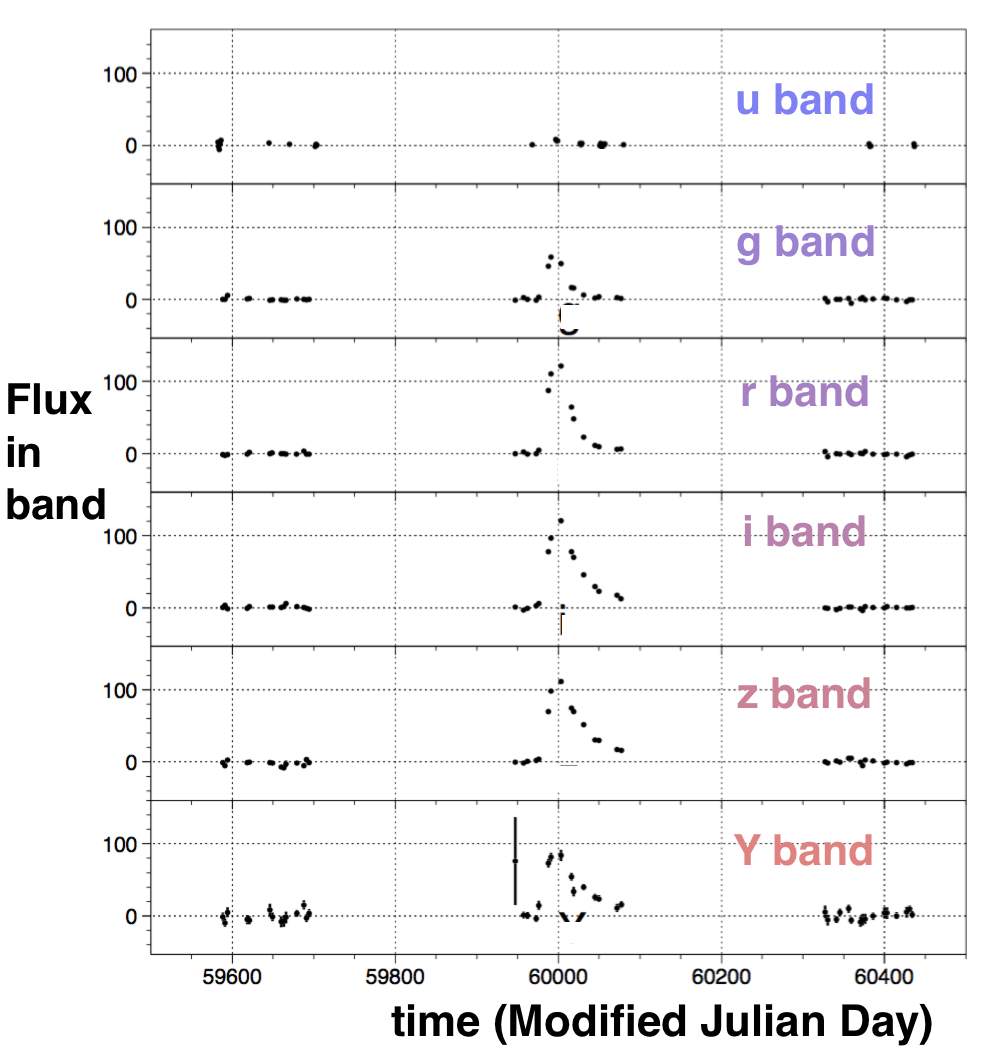
\includegraphics[scale=0.4]{figures/lcplot_model01a.png}
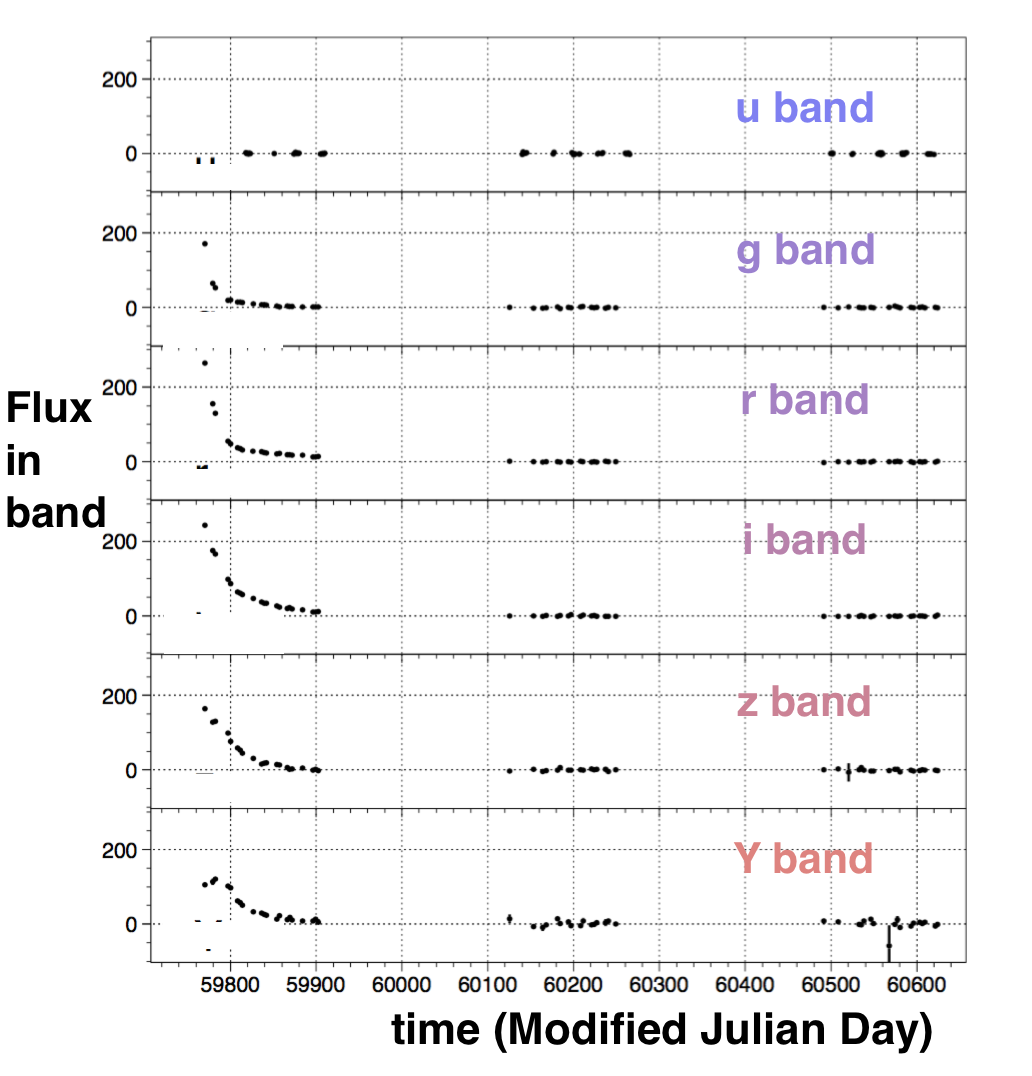
\includegraphics[scale=0.4]{figures/lcplot_model01b.png}
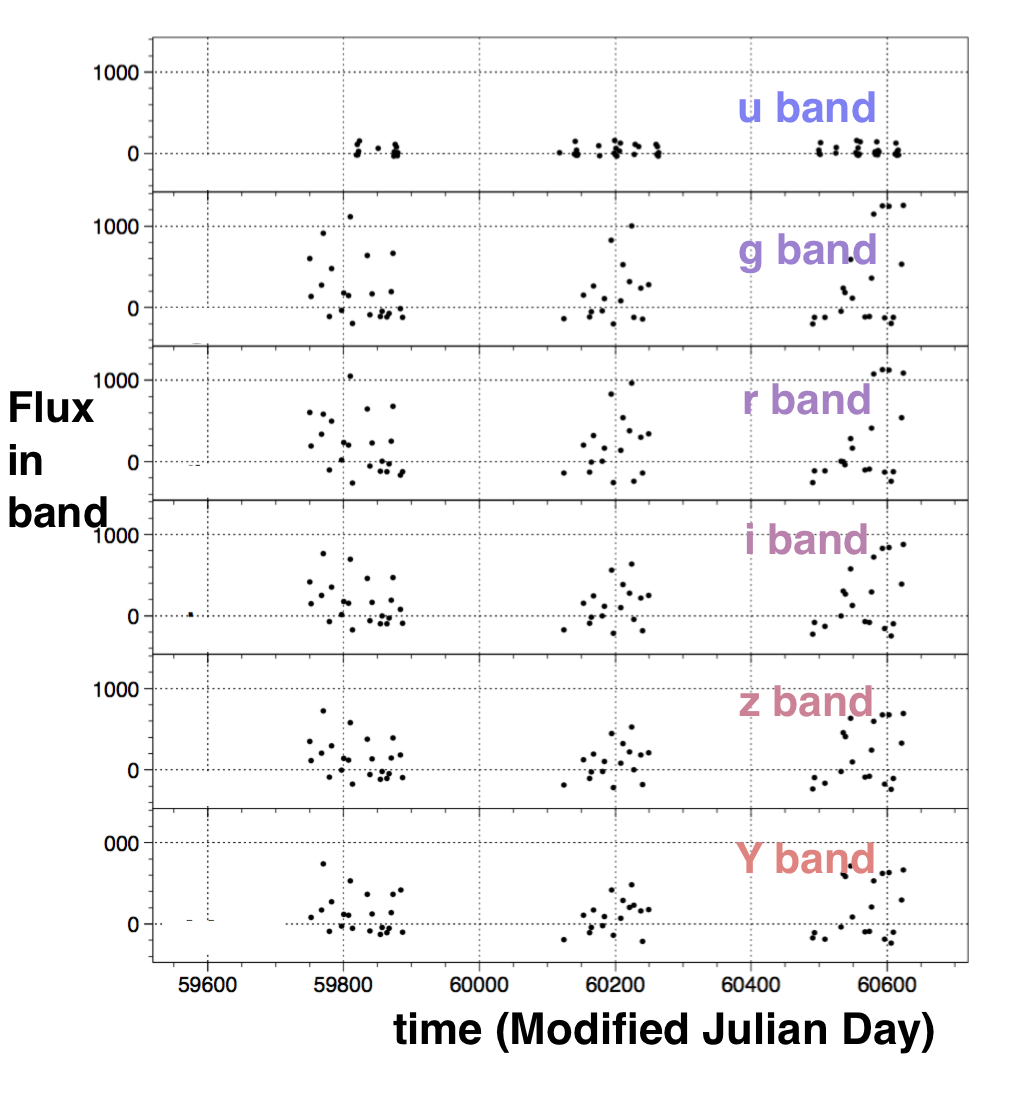
\includegraphics[scale=0.4]{figures/lcplot_model80.png}
\caption{Example light curves in the PLAsTiCC data set. The three example objects display different changes in flux with time that are typical of real objects. The top-right panel  illustrates that the brightening of the flux can occur near observation gaps, and therefore may not include the full time period of brightening (or fading) for the object. In addition, all three panels show that seasonal gaps and the instrument cadence of observations can introduce gaps in the light curve.\label{fig:lc}}
\end{center}
\end{figure*}



\section{Astronomy Background}
While we think of the night sky as static, it is filled with sources of light that vary in brightness on timescales from seconds and minutes to months and years. 

Some of these events are classified as   \textit{transients}, and are the
observational consequences of a large variety of astronomical phenomena. 
For example, the cataclysmic event that occurs when a star explodes generates a 
bright `supernova' signal that fades with time, but does not repeat.
Other events are classified as \textit{variables}, since they vary repeatedly in brightness in a periodic 
(or aperiodic) fashion.
% and originate from physical process governing high density regions of the Universe such 
Variable objects include emission from active galactic nuclei (AGN) at the hearts of galaxies, 
pulsating stars know as Cepheids,
and eclipsing binary stars that alternate blocking out each other's light from view.


These transient objects can provide important clues about themselves and their environment - as well as the evolution of the universe as a whole. For example, measurements of type Ia supernovae light curves provided the first evidence of accelerated expansion of the Universe, which might be caused by dark energy.

Each type of transient and variable provides a different clue that helps us study how stars evolve, the physics of stellar explosions, the chemical enrichment of the cosmos, and the accelerating expansion of the universe.  Therefore, the proper classification of transients is a crucial task in observational astronomy - specially in light of the large data volumes expected for the next generation of astronomical surveys - which includes LSST.

The question we address in this challenge is: \textit{how well can we classify astronomical transients and variables from a  light curve data set designed to mimic the data from LSST?} Crucially, the classification will occur on a large test set, but the training data will be a small, and poorly representative training set, to mimic the challenges we face observationally.

\subsection{Different Methods for observing Astronomical Objects}
\label{subsec:observmethods}
Here we give more detail on LSST, and the challenge at hand. The two modes for characterising light from astronomical objects are called `spectroscopy' and `photometry.'

Spectroscopy measures the flux per wavelength interval and is the modern equivalent of using a prism to separate a beam of light into a rainbow of colours. It is a high precision measurement which allows us to identify emission \& absorption features indicative of specific chemical elements present in the object.  Spectroscopy is also the most accurate and reliable tool that enables classification of astronomical transients and variables. Despite being paramount for the classification task, spectroscopy is an extremely time consuming process - with integration times ranging from 20 minutes to a few hours depending on the telescope and brightness of the source.

Given the volume of data expected from the upcoming large scale sky surveys, obtaining spectroscopy for every object is not feasible. An alternative approach is to take an image of the object through different `filters', where each filter selects light of a specific colour, or wavelength range. 
For LSST there are six filters denoted $u,g,r,i,z,Y$, which select light from 
ultra-violet ($u$), green ($g$), red ($r$), and three near-infrared filters ($izY$).
The filter efficiency vs. wavelength is shown in Fig.~\ref{fig:filters}.
For reference, the human eye is sensitive to light in the $g$ \& $r$ bands.
The flux of light in each filter, measured as a function of time, is a light curve.
Classification is performed on these light curves. 
While a spectrum contains thousands of measurements in small wavelength regions, 
the light curve data includes at most six measurements (1 per filter) at any given time. 
The challenge is to classify objects with the highly compressed light curve information. 
Compared with spectroscopy, the advantage of measuring light curves is that 
we can observe objects that are much further away and much fainter. In addition,
light curves from LSST can be measured over half the sky, a much larger region
than spectroscopy can cover.


% Photometry records how bright the source is at a given moment. The photometric information is encoded as the flux (energy from the object). The photometric light curve has six pieces of information, namely the flux in six wavelength bands (named $ugrizY$) at any moment in time.
% These photometric wavelength band fluxes are the integrals of the spectrum over the filter bandpasses of atmosphere and of the instrument divided by the energy of photons in the central wavelength of the filter. A sequence of photometric observations made at different times is called a light curve. It measures how the energy of the source evolves with time and can also be used to characterize different types of astronomical transients. As a consequence, for each object we will have a number of light curves in each filter (or band). Wavelengths are measured in units of Angstrom ($\AA$), where $1\AA = 10^{-10} m.$ Each band corresponds to a `color', with a width of around 1000 $\AA$, with the full set ranging from $3000\AA$ (blue light) to $9000\AA$ (near infrared light).

Beware that observations are sometimes degraded by moonlight, twilight, clouds, and wind.
These degradations result in larger flux uncertainties, 
and this information is included in the light curve data (see Sec 3 below).

In addition to providing light curves, two other pieces of information are provided
for each object.
First is a proxy for distance called `redshift', where more distant objects have a larger redshift.
The training set includes accurate redshifts from the object, but the test data redshifts
are approximate measurements based on $ugrizY$ filter measurements from the `host galaxy' 
of the object. While transients brighten and fade, the host galaxy fluxes don't change
and can thus be measured before an object's light curve starts, or after it has faded.
Beware that a few percent of the test data redshifts are catastrophic, 
meaning that some redshift uncertainties greatly under-estimate the difference
between measured and true redshift.


The redshift effect is illustrated in Fig.~\ref{fig:filters}.
The black curve shows a {\it nearby} Type Ia supernova spectrum at a redshift of 0.01,
corresponding to a distance of 140 million light years. 
While the term `nearby' may seem strange in this case, this distance is 
indeed nearby when compared with the whole range of cosmic distances.
Visual inspection of the supernova spectrum and the filter efficiencies shows that
the maximum flux (spectrum summed over filter) is in the 
green ($g$) filter.
The dashed curve shows a spectrum from a more distant Supernova, 
corresponding to a redshift of 0.5, or 5.1 billion light years 
away.\footnote{The relation between distance and redshift is not linear, 
but is a function derived from General Relativity which depends on the properties of 
dark matter and dark energy.}  % end footnote
The maximum flux is now shifted to the red ($r$) filter.
As the redshift and distance increase, the maximum flux appears
in a redder filter: hence the term `redshift.'

The second piece of information is related to extinction from our Galaxy, 
known as the Milky Way. While our light curve measurements correct
for the atmosphere and telescope transmission, we do not correct for
absorption of light travelling through Milky Way `dust' on its way to Earth.
This absorption is strongest in the ultra-violet $u$-filter, and weakest
in the infrared filters ($izY$). 
The data parameter has a strange name called `MWEBV', which is an 
astronomical measure of how much redder an object appears compared
to a Milky Way without dust. 
Larger MWEBV values correspond to more Milky Way dust,
and objects appearing redder.


\begin{figure}
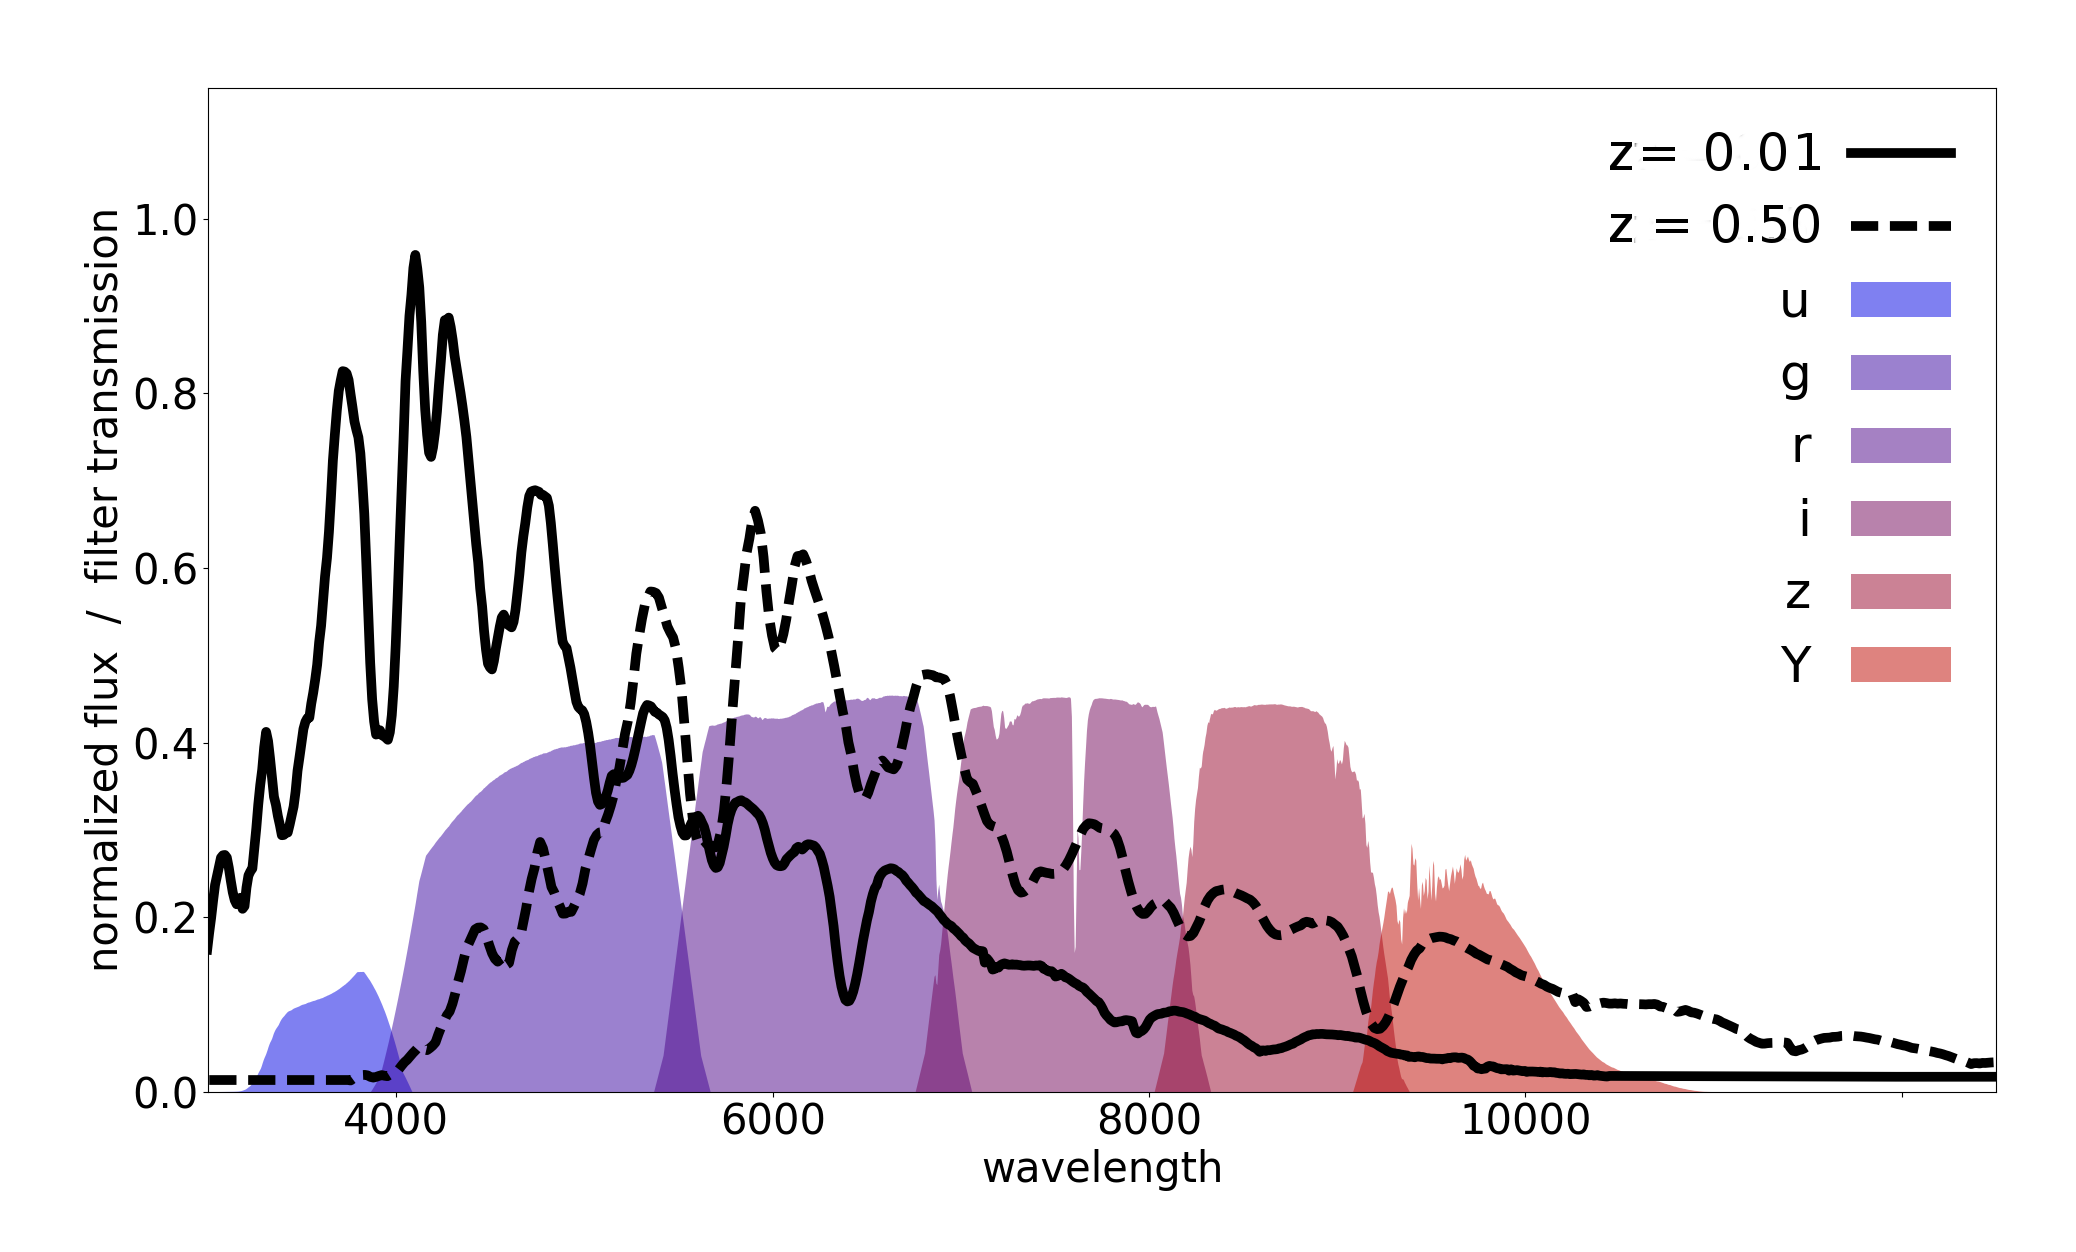
\includegraphics[width=\textwidth]{figures/spec_filters.png}
\caption{Shaded regions show $ugrizY$ filter efficiency vs. wavelength.
Each measured filter flux is a sum of the photons collected within the wavelength range.
Black curve shows a spectrum for a nearby Type Ia Supernova at redshift 0.01;
dashed curve shows a spectrum for the same object at redshift 0.5~.
The dashed spectrum {brightness is much lower than the solid spectrum, and has thus been scaled} to see its shape relative
to the solid spectrum.}
\label{fig:filters}
\end{figure}



%Unlike spectroscopy, photometry measures light from a large wavelength range simultaneously, and therefore collects more photons during observation, making it possible to measure light from objects at greater distances than with spectroscopy. For an object of given brightness (luminosity), the flux received on earth decreases with the distance to the object as

%Hence if the intrinsic luminosity of an object is known, then its flux can be used to determine the distance to the object. This distance is an important tool in classification, since different objects are more likely to be found within or outside of our own galaxy.

%When working in magnitudes, we connect the distance to the magnitudes via the distance modulus $\mu$:

%\begin{equation}
%\mu = m-M = 5\log_{10} d_L + 25,
%\end{equation}

%where $M$ is the (unknown) intrinsic brightness of the object, $d_L$ is measured in megaparsec (Mpc), $c$ is the speed of light and $H_0 \simeq 70$ km/s/Mpc is the Hubble constant. Programs exist to fit for the distance modulus $\mu$ given the light curve points and models for the type of object.


%The final connection is model cosmic distances through an expanding universe cosmological model. In such a cosmology of the universe, the connection distances to objects comes through the redshift, $z$. Redshift is an empirical quantity that is defined by measuring the difference in the observed wavelength $\lambda_o$ of a given feature (e.g. in the spectrum described above) compared to the emitted wavelength $\lambda_e$, or

%\begin{equation}  z = \frac{\lambda_o - \lambda_e}{\lambda_e}. \end{equation}

% Just like the Doppler affect that acts on sound waves, redshifting is the analog for light. Using a spectrum to determine the redshift of an object gives the most precise result (with the smallest error $\sigma_z$). However photometry of the galaxy that `hosts' the object, can also be used to determine a redshift for an object, the so-called photometric redshift, with a larger uncertainty. 
% Photometric redshifts can include so-called catastrophic failures, where the redshift of the object is misassigned. These errors are rare (roughly $2\%$ of the total number of objects), however they can pose serious problems for classification of objects.

%The distance modulus is connected to the cosmological model of the universe as a function of redshift $z$ and the components (like the amout of matter and energy) of the universe. We do not expect participants of this challenge to compute these functions, and will provide the distane modulus and error on the modulus as if the data had been run through a light-curve model fit.

%\subsection{The Large Synoptic Survey Telescope (LSST)}
%LSST is an ambitious telescope project under construction in Chile, scheduled to begin observations in 2022. With its powerful camera and wide field of view, it will be able to scan the whole sky visible from Chile once every three days. LSST will produce an unprecedented number of light curves by comparing images from day to day and looking for new objects not seen previously, and measuring the flux in those images. Once these transients are detected, we rely on agreements with other telescopes in order to acquire a small number of spectroscopic observations.


%We will describe the data in the following sections, and discuss the metrics used to classify objects in a separate note.
%\end{document}

\section{The data}
\label{sec:thedata}

The light curve data for each object consists 
of a time series of fluxes in six filters (ugrizY), 
with non-uniform  time sampling.
The {\plasticc} data is provided in the form of a HDF5 file, which has two kinds of information. The first
is a table listing each astronomical source in the data indexed by a unique identifier 'objid' which is a string. Each row of the table lists the properties of the source as follows: 
\begin{itemize}
\item {\tt objid}: the Object ID, unique identifier, string
\item {\tt ra}: right ascension, sky coordinate: co-longitude, units are degrees
\item {\tt decl}: declination, sky coordinate: co-latitude, units are degrees
\item {\tt mwebv}: a property of the Milky Way dust along the line of sight to the astronomical source, and is thus a function of the sky coordinates of the source {\tt ra, decl}. This is used  to determine a {\passband} dependent dimming and redenning of light from astronomical sources as described in subsection~\ref{subsec:observmethods}.
\item {\specz}: the spectroscopic redshift of the source. This is an extremely accurate measure of redshift, 
    and is not measured for the test sample. Hence, these values are null in the test data.
\item {\hostphotoz} : The photometric redshift of the host galaxy of the astronomical source. While this is meant to be a proxy for {\specz}, there can be large differences between the two and should be regarded as a far less accurate version of {\specz}. 
\item {\hostphotozerr} : The uncertainty on the {\hostphotoz}
\item {\class} : The class of the astronomical source as a string. (currently this variable is called `sntype' and will be changed in future)
\end{itemize}

The second table of information about the transients is its brightness as a function of time in different {\passband}s, ie. light curve data. Each row of this table corresponds to an observation of the source at a particular time and passand.  This table includes the following information
\begin{itemize}
\item {\tt mjd}: the time (float) in Modified Julian Date (MJD) of the observation with a unit of day.
\item {\passband} : The specific LSST {\passband} string: u, g, r, i, z, Y in which it was viewed. 
\item {\tt flux}: the measured flux (brightness) in the {\passband} of observation as listed in the {\passband} column. This is a float.
\item {\tt fluxerr}: the uncertainty on the measurement of the {\tt flux}  listed above.
\item {\tt photflag}: ignore.
\end{itemize}

A few caveats about the light curve data are as follows:
\begin{itemize}
    \item \textbf{Negative Flux} Due to statistical fluctuations and the way the brightness is estimated, the flux may be negative for dim sources, where the true flux is close to zero. 
    \item \textbf{saturated observations} The light curves include `saturated' observations of sources, where the source is
too bright to obtain a measured value. In such cases, the {\tt flux} is set to 0., and the {\tt fluxerr} is set to 10,000,000. Such an observation may not yield a value of {\tt flux}, but it indicates that the source was extremely bright rather than extremely dim at the time of observation. 
\item \textbf{Observing Cadences} The objid string has two prefixes ‘DDF’ and `WFD.’  DDF corresponds to
“Deep Drill Fields” over a small area of sky, but with very high quality 
light curves. “WFD” corresponds to “wide-fast-deep” over a very large 
sky area, but with lower quality light curves.

\end{itemize}

\clearpage
%It is possible that the distribution of properties (as found in the header table) could be different for different classes of astrophysical sources. For example, sources that are extremely dim, may only be found in our own galaxy the Milky Way, and thus their redshifts will be close to zero, and their locations are likely to be clustered around the parts of the sky where the Milky Way is densely populated. Sources that are somewhat brighter, but still too dim to be see from large cosmological distances may be found at low redshifts only. On the other hand, extremely bright sources which are visible for extremely large distances may tend to be found at higher redshifts due to larger physical volume at high redshifts. On the other hand, the signature of a particular class of astrophysical source is to be found in its light curve, which is a degraded and compressed version of its spectral evolution. 

\subsection{Obtaining the data and Scoring a classification}
The header table is located in the sample HDF5 file at the path {\header}, while the light curve is stored at the path `objid' in the sample HDF5 file. As part of the challenge, we provide an example Jupyter notebook to read in the data from an HDF5 file, and a notebook to compute the metrics for the challenge.

\subsection{Training And Test Data}
The training data follow the description above and have the properties and light curves of a set of {\numObjectsTraining} astronomical sources and are meant to represent the brighter objects for which obtaining expensive spectroscopy is possible. The test data represent all of the data which have no spectroscopy.
Therefore, the test data has `NULL' entries for the two columns {\specz} and {\class}. Moreover, for this reason their properties are \textbf{non-representative} of distributions of the
the test data set. The training data are mostly comprised of nearby, low redshift, brighter samples while the test data contain higher redshift, fainter and more distant objects. Therefore, there are objects in the test data that do not have counterparts in the training data.


% ----------------------------------------------------------------------

\section{Challenge participation}
\label{sec:conclusion}
{\plasticc} challenge entries are required to classify each of the sources in the header file of the test data set  based on their properties and light curves. The classification must be done though the assignment of probabilities $P_{ij},$ 
%$P(\rm{class}\vert\rm{data}_{i}, \rm{training-data}, \rm{knowledge}),$ 
the probability that the $i\rm{th}$ source in the test data is a member of the class $j$ based on the combination of properties and light curve data for the object, the training data set, and any outside knowledge the participant may have acquired elsewhere. To specify the entry for a single source, the participant must provide the probabilities of that source belonging to each of the mutually exclusive (non-overlapping) `{{\numclasses}}  classes in the training set, and of not belonging to any of the classes in the training set and therefore denoted by the {\tt others} class. High values of $P_{ij}$ for a particular class $j$ and object $i$ indicate that the participant believes that the ith source is likely to be a member of the $j$th class. 
As true probabilities, the quantities $P_{ij}$ must satisfy the following criteria:
\begin{eqnarray*}
0.0 \leq P_{ij} \rm{knowledge}) \leq 1.0 \qquad \forall i, j \nonumber \\
\sum_{j} P_{ij} = 1.0 \qquad \forall i
\nonumber
\end{eqnarray*}
For a {\plasticc} entry to be valid, it must have these probabilities for each class and astronomical source, ie. an entry cannot leave out probabilities on any source, or class. To win the challenge, the entry must be a valid entry and minimise the PLAsTiCC metric score (which is described in a separate note included in this challenge). 
For a participant using a classifier which decides that an object is of a particular class rather than provide probabilities, the participant has to use their own prescription to define probabilities. For example, a source classified as the first class may be given a probability of 1.0 and all other classes probabilities of 0.0, or the first class may be assigned 0.9 and all other classes may be given uniform probabilities so that the probabilities sum to unity. 

For example, if the challenge was to classify a set of 3 observations into two classes of `star' or `galaxy' classes (and an `other' class), the returned classification table would be $3x3$ matrix:

\begin{table}[htbp!]
\begin{center}
\begin{tabular}{|c|c|c|c|}
Object ID & $P(star)$ & $P(galaxy)$ & $P(other)$ \\
\hline
1 & 0.6 & 0.3 & 0.1\\
2 & 0.3 & 0.3 & 0.4\\
3 & 0.55 & 0.4 & 0.05\\
\end{tabular}
\caption{An example classification table for a challenge to classify 3 objects into 3 classes}
\end{center}
\end{table}

The {\plasticc} team involved in validating the data will not be able to participate in the challenge directly, and will only publish classifications on the data once the challenge has completed. Some {\plasticc} team members involved in defining metrics will participate in the challenge, but they have not seen any {\plasticc} information about the models or the data.

% ----------------------------------------------------------------------

\subsection{Acknowledgments}
The {\plasticc} data relies on numerous members of the astronomical community to provide models of astronomical transients and variables. These models will be described in a paper to be published once the challenge is complete. While we cannot thank them by name at this stage (as this could identify the models included in the challenge), we acknowledge their contributions anonymously at this stage. This work was supported by an LSST Corporation Enabling Science grant, and a Dark Energy Science Collaboration Workshop support grant.

%%% Here is where you should add your specific acknowledgments, remembering that some standard thanks will be added via the \code{desc-tex/ack/*.tex} and \code{contributions.tex} files.

%This paper has undergone internal review in the LSST Dark Energy Science Collaboration. % REQUIRED if true

%
 % Standard papers only: author contribution statements. For examples, see http://blogs.nature.com/nautilus/2007/11/post_12.html

% This work used TBD kindly provided by Not-A-DESC Member and benefitted from comments by Another Non-DESC person.

% Standard papers only: A.B.C. acknowledges support from grant 1234 from ...

\input{desc-tex/ack/standard} % also available: key standard_short

% This work used some telescope which is operated/funded by some agency or consortium or foundation ...

% We acknowledge the use of An-External-Tool-like-NED-or-ADS.

%{\it Facilities:} \facility{LSST}

% Include both collaboration papers and external citations:
%\bibliography{main,lsstdesc}

\end{document}

% ======================================================================
